\documentclass[screen]{beamer}
\usepackage[T1]{fontenc}
\usepackage[utf8]{inputenc}
\usepackage{multimedia}

\usepackage{algorithm}
\usepackage{algorithmic}
\usepackage{bm}


% Bruk NTNU-temaet for beamer (her i bokmålvariant), alternativer er
% ntnunynorsk og ntnuenglish.
\usetheme{ntnuenglish}
 
% Angi tittelen, vi gir også en kortere variant som brukes nederst på
% hver slide:
\title[Eksempelforedrag]%
{COOL AND AWESOME TITLE}

% Denne kan du også bruke hvis det passer seg:
%\subtitle{Valgfri undertittel}

% Angir foredragsholder, også en (valgfri) kortversjon i
% hakeparanteser først som kommer nederst på hver slide:
\author[aut]{Aga, Kristian \\ Berge, Runar L. \\ Klemetsdal Øystein S.,\\
	Myrvoll Nilsen, Eirik \\ Selle, Maria.
}


% Institusjon. Bruk gjerne disse slik det passer best med det du vil
% ha.  Valgfri kortversjon her også
%\institute[NTNU]{Institutt for matematiske fag}

% Datoen blir også trykket på forsida. 
\date{November 23., 2015}
%\date{} % Bruk denne hvis du ikke vil ha noe dato på forsida.

% Fra her av begynner selve dokumentet
\begin{document}

% Siden NTNU-malen har en annen bakgrunn på forsida, må dette gjøres
% i en egen kommando, ikke på vanlig beamer-måte:
\ntnutitlepage

\section*{Modelling}
\begin{frame}
    \frametitle[jaddA]{Inundation}
    \begin{enumerate}[\label = $\circ$]
        \item    owje
        \item    Jee
        \item    Hm
    \end{enumerate}
    \begin{block}{This is a textbox with meaningful equations}
        \begin{align*}
            rhs = lhs.
        \end{align*}
    \end{block}
\end{frame}

\begin{frame}
    \frametitle{Inundation}
    \begin{itemize}
        \pause
        \item    h1
        \pause
        \item    h2    
    \end{itemize}
    \pause
    \begin{block}{This is another textbox with meaningful equations}
        \begin{align*}
            rhs = lhs.
        \end{align*}
    \end{block}
\end{frame}

\section*{Numerical solutions}

\begin{frame}
    \frametitle{Mimetic finite difference/ forward difference scheme (M(FD)$^2$S)}
    \begin{align*}
        & \Delta \phi = 0 \\
        & \eta_t + \nabla\phi\cdot \big(\eta_x, \eta_y, - 1\big) = 0 \\
        & \phi_t + \frac{1}{2}|\nabla \phi |^2 + g\eta = 0.
    \end{align*}
\end{frame}

\begin{frame}
    \frametitle{Calculating $\nabla \phi$}
	\only<1-1>{
	\begin{figure}[b]
		\centering
		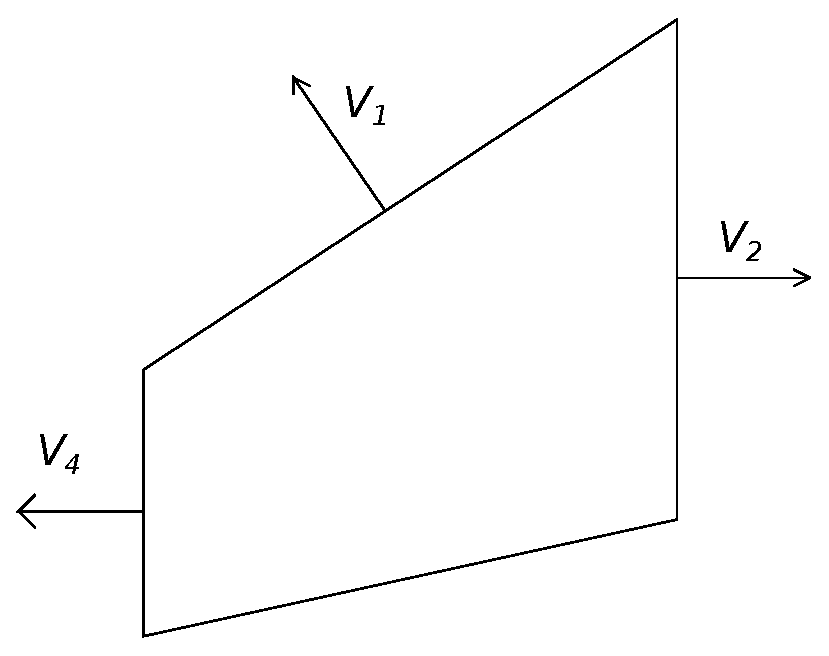
\includegraphics[width=0.5\textwidth]{fig/calculatingFlux.eps}
	\end{figure}
	}
\end{frame}

\begin{frame}
	\frametitle{Numerical Solutions of the Shallow Water Equation}
	\begin{block}{The System of Equations}
		\begin{align*}
		\begin{array}{c c}
		V_t + (u+\sqrt{\eta})V_x = 0, & V = u + 2 \sqrt \eta\\
		U_t + (u-\sqrt{\eta})U_x = 0, & U = u - 2\sqrt \eta
		\end{array}
		\end{align*}
	\end{block}
\end{frame}
\begin{frame}
	\frametitle{Numerical Scheme}
	\only<1-1>{
	\begin{figure}[b]
		\centering
		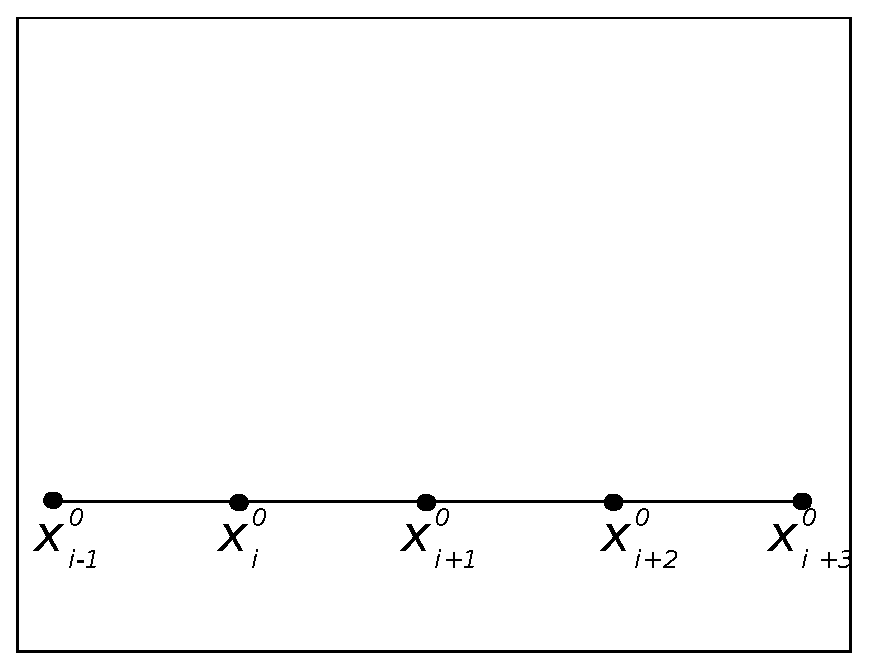
\includegraphics[width=0.7\textwidth]{fig/charWaveEq1stStep.eps}
	\end{figure}
	}
	\only<2-2>{
		\begin{figure}[b]
			\centering
			\includegraphics[width=0.7\textwidth]{fig/charWaveEq2ndStep.eps}
		\end{figure}
	}
	\only<3-3>{
		\begin{figure}[b]
			\centering
			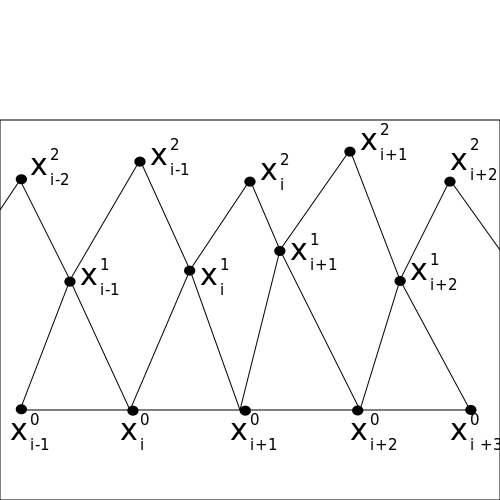
\includegraphics[width=0.7\textwidth]{fig/charWaveEq3rdStep.eps}
		\end{figure}
	}
\end{frame}

\end{document}